\chapter{基于点云语义分割域适应的主动混合策略}
\thispagestyle{others}
\pagestyle{others}
\xiaosi

    \section{本章引言}
    本章主要介绍基于点云语义分割域适应的主动混合策略。该方法通过将基于原型指导的主动学习方法和本节所提出的主动混合策略进行深度结合,进一步提升了主动域适应方法的结果。接下来,下文将分别从方法提出的研究动机及主要贡献、方法的具体组成和实现细节,以及实验分析评估等方面,对所提出的方法进行全面阐述。 

    \section{研究动机及贡献}
    % 首先说研究背景和问题,再说一些解决的方法,然后提一下前者怎么做的,后者怎么做的
    % 第二就是说一些文章,他们是怎么使用这些方法解决问题的
    % 第三就是提上述文章方法的不足,
    % 核心点是:主动域适应中主动学习与mixing的结合不够深入,仍然有很大的探索空间。
    % 背景现状(标注问题)-> 一些现存的方法 -> 域适应中和主动学习以及mixing的方法 -> mixing方法构建中间域,举例一些方法,然后这些方法在mixing的不足,尽管如此,但是mixing与主动学习在域适应的结合是从没有过,或者说mixing与主动学习的结合从未有过探索,但是它们却有着巨大的探索价值 -> 我们从上一章节看到了mixing带来的提升,但是基于AL的mixing还有更大的探索空间,对于这两个的结合的探索仍然缺乏。
    % 一些研究者将mixing用于半监督域适应中
    % 主动域适应的问题,以及mixing却可以为之互补。
    % 域适应中有主动域适应和一些基于无监督或者半监督的域适应。
    % 然而在域适应中主动学习方法和mixing
    % 提及一些主动域适应的方法以及已无监督域适应的一些mixing方法
    % 在。。中,。。。使用mixing。。。的提升了模型性能,域适应中。。。使用mixing提升了性能,在。。。中通过主动域适应得到了很好的解决,mixing和主动学习分别为标注问题默默贡献着。或者直接说主动域适应的问题,然后引出一些mixing方法的好处,可以完美的进行结合。
    % 科技的进步使得点云雷达数据的获取变得更加容易,深度学习技术的发展则使得点云语义分割任务得到了快速进步,一些优秀的模型接踵而至,并取得了令人瞩目的结果。但是,这些优秀模型都是基于全监督模式下的,需要点云样本进行逐点的标注,而点云标注则是一项耗费人力物力的艰巨任务。为了缓解这以问题,一些优秀的方法被提出,而域适应就是其中之一。在无监督和半监督域适应中,一些方法独出心裁,使用mixing的方法构造中间域来学习特征的不变性,进而解决域偏差问题。polarmix[]。提出将不同的雷达线速进裁剪并混合。CoSMix[]。将指定语义类别的源域点和伪标签置信度高于阈值的目标点进行过交换混合。而主动域适应[HPML、CLUE、SDM]则是通过选择对缩减域偏差帮助最大的目标点,并进行标注后以提升模型的性能。
    科技的进步使得获取点云雷达数据变得更加容易,而深度学习技术的发展则推动了点云语义分割任务的迅速提升,涌现出一系列优秀模型并取得了显著成果。然而,这些模型大多基于全监督模式,需要对点云样本进行逐点标注,这是一项耗费大量人力物力的艰巨任务。为缓解这一问题,研究者们提出了多种方法,而域适应就是其中一种有效的策略。在无监督和半监督域适应中,一些方法巧妙地使用混合策略构造中间域,以学习特征不变性,进而解决域偏差问题。Polarmix\upcite{xiao2022polarmix}方法则是沿方位角分割并混合不同扫描的点云区域,在域适应中混合的则是不同数据集下的同角度点云区域。LaserMix\upcite{kong2023lasermix}方法通过裁剪并混合不同雷达线束实现源和目标的混合。
    % CoSMix\upcite{saltori2022cosmix}方法则交换并混合源域中指定语义类别的点与目标域中伪标签置信度高于阈值的点。
    此外,主动域适应方法\upcite{CLUE,HPML,SDM}通过主动选择对减小域偏差最有帮助的目标点进行标注,从而提升模型性能。 

    尽管上述算法各自以不同方式缓解了标注问题,提升了分割模型的性能,但在域适应中,主动学习与混合策略的结合尚未得到深入研究。无论是在图像还是三维点云领域,混合策略和主动学习通常独立应用,分别为减少标注需求做出贡献。然而,现有的混合方法若直接应用于主动域适应,可能存在以下问题:1)数量不均衡导致的域偏差问题。现有的混合方法多基于同一数据集或大量伪标签,特点是场景连续且点数丰富。然而在域适应中,源域和目标域存在域偏移,主动学习预算下选择的点数量有限。若直接应用这些混合方法,可能导致模型过度学习源域信息,阻碍对目标域信息的提取,最终导致次优结果。因此,在主动域适应中,保持源域和目标域信息的平衡可能比场景连续性更为重要。主动学习选点导致的语义类别不平衡问题。大多数主动学习选点策略基于不确定性。在实际标注前,无法确定所选子集的类别分布是否均衡。尽管一些方法通过伪标签预判类别,但这基于模型不可靠的预测,在域适应任务中可能不适用。此外,现有的混合方法未考虑逐点的语义类别平衡问题。因此,如何使主动学习选择的目标子集与源数据混合后的训练子集在类别分布上尽可能平衡,仍是一个普遍存在的问题。
    针对上述问题,本章进一步探讨了主动学习方法与混合策略在域适应任务中的深度结合。在该方法中,延续前章使用基于原型指导的主动学习与混合策略(Mixing)相结合的基础框架。在此基础上,提出了面向点云语义分割域适应的主动混合策略。其包括两个模块:源-目标数量平衡模块旨在解决数量不均衡导致的域偏差问题;类别平衡主动混合模块用于解决主动学习选点导致的语义类别不平衡问题。这两个模块有效地实现了主动学习与Mixing方法的深度结合,进一步提升了模型的分割性能。
    % 虽然上述算法都通过自己的方式解决了标注问题,使得分割模型有了一定的提升,但是对于域适应中主动学习和mixing的结合并未有人进行过深入的探索,无论是在图像还是三维点云领域,mixing和主动学习独立且分别为缓解标注问题默默贡献着。而现存的mixing方法如果直接运用到主动域适应中可能存在以下问题:1)数量不均衡而导致域偏差问题,由于之间的mixing方法更多的是基于同一数据集或者大量的伪标签的前提下的,因此这些方法有着共同的特点:场景连续且点数更多。而在域适应中,目标域和源域之间存在域偏移问题,并且主动学习预算选择的点非常少,因此如果直接将这些mixing方法运用到主动域适应中,可能会导致模型因学习到更多源域信息而阻碍对目标域信息的提取,得到次优的模型结果。因此在主动域适中,场景的连续可能并不是那么重要,相同的源-目标域信息可能才是进一步提升模型性能的最佳混合方法。2)主动学习选点导致的语义类别不平衡问题。目前为止,大多数主动学习的选点策略都是基于不确定性的,在真实标注之前,我们无法得知最终选择的子集的类别分布是否均衡,虽然有一些方法通过伪标签的方式提前预判选择的类别,但这仍然是基于模型的不可靠预测的伪标签,在域适应任务中可能并不适用,现有的mixing未考虑逐点即语义类别平衡的问题,因此存在一个普遍的问题,
    % 如何使得主动学习选择后的目标子集与源数据混合后的训练子集是类别分布尽可能得平衡。对于上述问题,本章节进一步探索了用于域适应任务的主动学习方法与mxing深度结合。在该方法中,首先将提出的基于原型指导的主动学习与Mixing结合形成了基础结合框架,并基于该框架提出了面向点云语义分割域适应的源-目标数量平衡算法和类别平衡主动混合算法。源-目标数量平衡算法解决数量不均衡而导致域偏差问题,类别平衡主动混合算法用于解决主动学习选点导致的语义类别不平衡问题。两个算法有效的完成了主动学习和mixing方法的深入结合,并进一步提高了模型分割的性能。
    
    本章研究的主要贡献如下:

    1)提出了源-目标数量平衡模块,通过选择与目标域样本中标注数量相同的源点进行混合构建中间域,解决了因数量不平衡导致的域偏差积累问题,进一步提高了混合中间域的有效性。

    2)提出了类别平衡主动混合模块,利用在源-目标数量平衡算法得到多个候选源点混合子集,计算并选择与标注的目标域混合后类别分布最为均衡的子集进行Mixing,借助源域数据实现主动选点的类别平衡,进一步提升了主动学习的有效性。

    3)根据提出的两个算法模块实现了主动学习与Mixing的深入结合,得到了深度融合主动混合的点云语义分割域适应框架,分割表现领先于所有现存域适应方法。

    % 为了更进一步提升在主动域适应中主动学习方法与Mixing的进一步结合,提出了基于点云语义分割域适应的主动混合策略。在该方法中,首先将提出的基于原型指导的主动学习与Mixing结合形成了基础结合框架,并基于该框架提出了面向点云语义分割域适应的源-目标数量平衡算法和类别平衡主动混合算法,两个算法有效的适配了主动域适应中的主动学习,减小了域差异和主动选择中类别不平衡则一普遍存在的问题,并进一步提高了模型分割的性能。

    \section{基于点云语义分割域适应的主动混合策略}
    在第三章中,设计了一个基于原型的主动学习方法,并初步尝试结合混合方法构建强健的中间域数据,以缩减域偏差,提升模型性能。然而,混合方法与主动学习的结合仍有广阔的探索空间。如何根据域偏差以及主动学习的特点来有效结合混合方法,仍是一个值得深入研究的问题。

    为了深入探讨混合(Mixing)方法与主动学习在域适应任务中的深度融合,本章在第三章提出的总体框架基础上进行了改进,改进后的框架如图\ref{fig:4-1}所示。该算法的基本流程主要由三个主要模块构成:%\ding{172}源域原型构建模块;
    \ding{172}源原型引导的数据选择模块(SPAL);\ding{173}源-目标数量平衡模块(STNB);\ding{174}类别平衡主动混合模块(CBAM)。为进一步实现两者的高效协同作用,从而获得更优的分割表现,本章对第三章的动态中间域构建模块进行了改进,分为两个模块:一是源-目标数量平衡模块,选择类别数量大于预设定值的源域帧,并从中筛选与所匹配的目标域帧标注点数平衡的候选子集;二是类别平衡主动混合模块,计算每个候选子集与目标域帧标注点混合后的类别分布熵值,选择熵值最大的候选源域子集,以构建类别相对平衡的中间域数据。

    通过上述改进,旨在实现混合方法与主动学习在域适应任务中的深度融合,进一步提升模型的分割性能。 
    \vspace{-0.1cm}
    \begin{figure}[h]
        \centering
        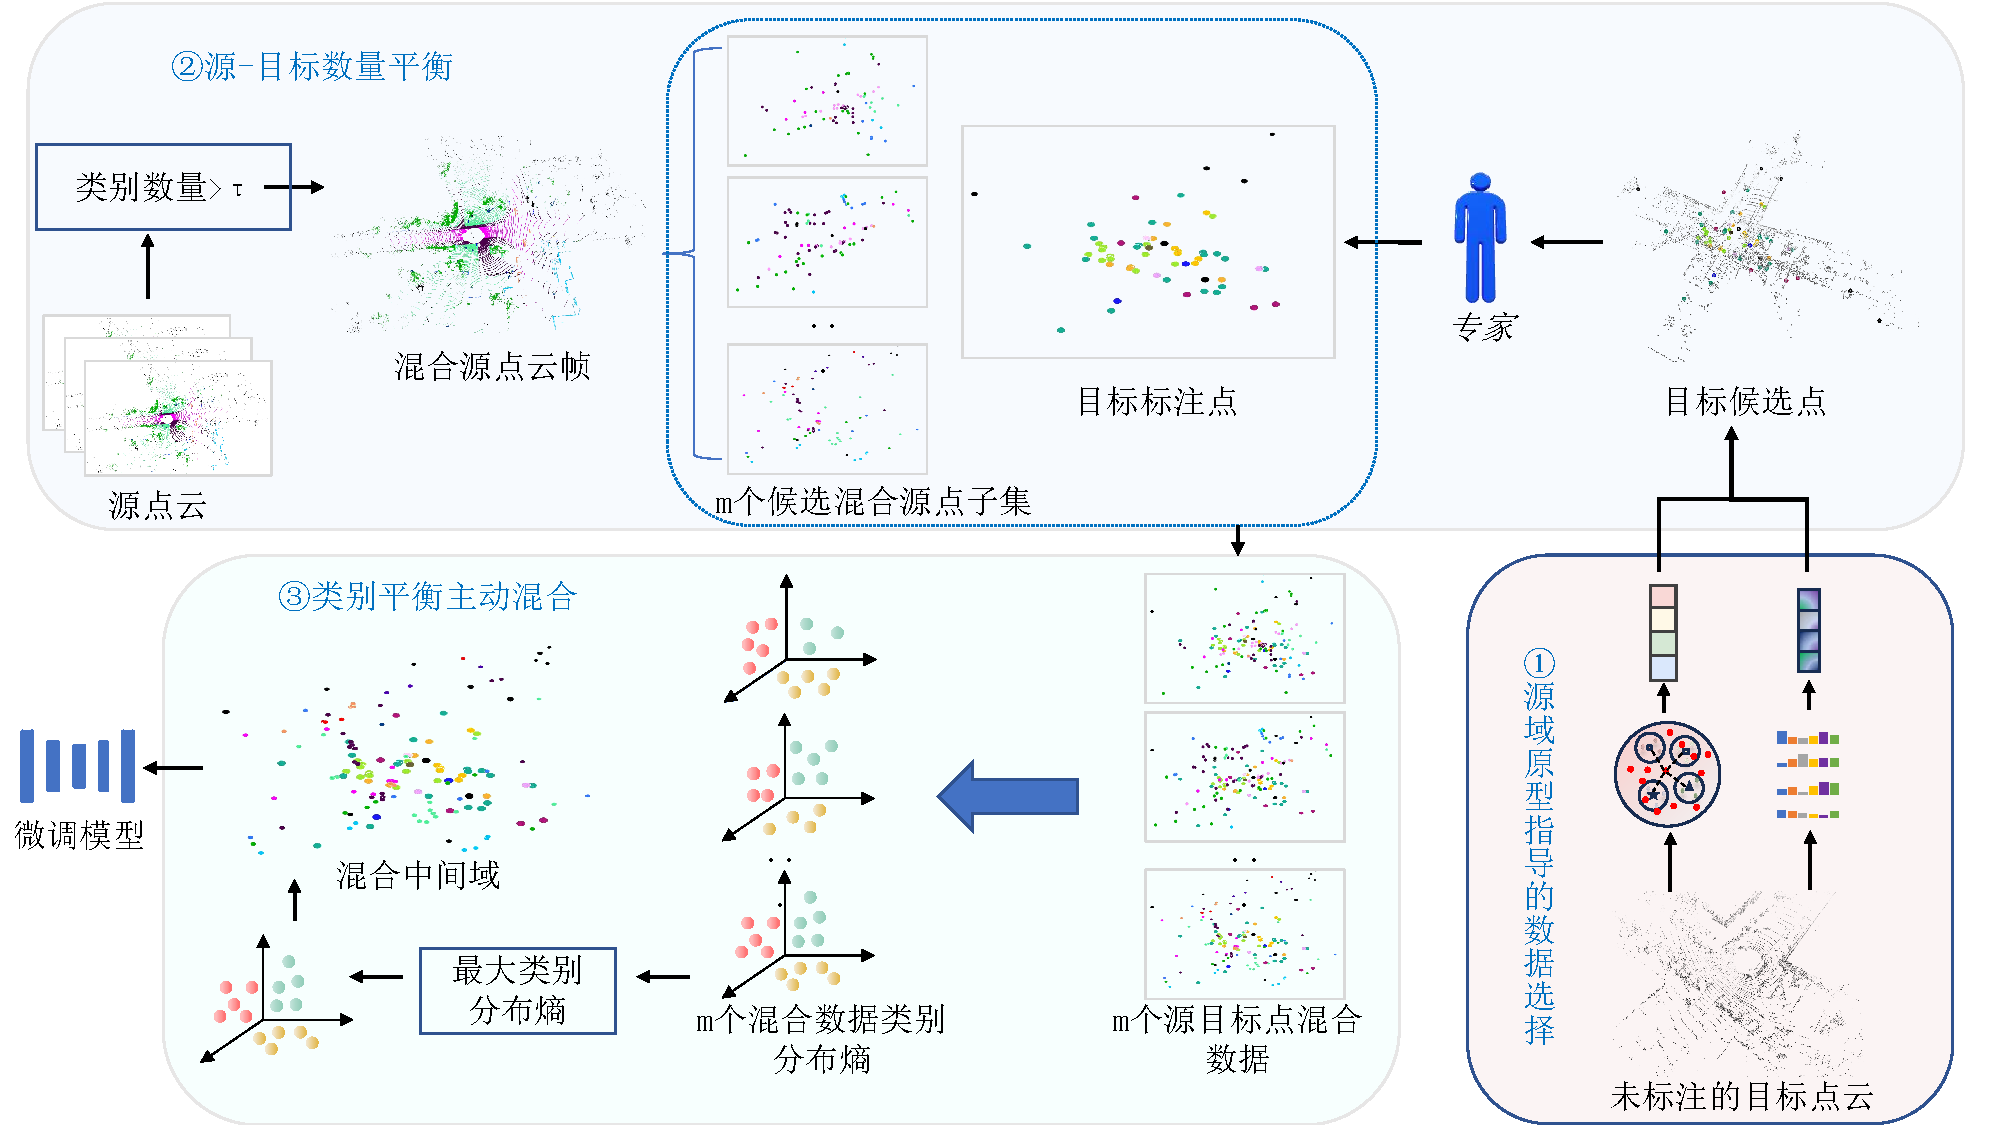
\includegraphics[width = \textwidth, scale=0.5]{ljx/figure/4-1framwork.pdf}
        \bicaption[\xiaosi 基于点云语义分割域适应的主动混合策略框架]{\wuhao 基于点云语义分割域适应的主动混合策略框架}{\wuhao Framework of active mixing for domain adaptation in point cloud semantic segmentation}
        \label{fig:4-1}
    \end{figure}
    \vspace{-0.35cm}
    % 为了探索mixing方法与主动学习在域适应任务上的深度结合,本章方法延续第三章的总体框架进行改进,改进后的框架如图 x-x 所示。算法基本流程主要由四个主要模块构成:\ding{172}源域原型构建模块,\ding{173}源原型引导的数据选择模块(SPAL),\ding{174}源-目标数量平衡模块以及\ding{175}类别平衡主动混合模块。在第三章中,我们设计了基于原型的主动学习方法,并初步探索结合Mixing方法构建出强壮的中间域数据,进一步缩减了域偏差,提升了模型的性能。然而对与mixing与主动学习的结合仍然有很大的探索空间。如何根据域偏差以及主动学习的特点来结合mixing仍然时一个可以探索的巨大问题。为了进一步形成两者间的高效促进作用从而获得更好的分割表现,本章方法在第三章的动态中间域模块进行了改进,分为了两个模块。一个是源-目标数量平衡模块:选择大于预设定类别数量的源域帧,并从中筛选与所匹配的目标域帧标注点数平衡的候选子集。另一个则是类别平衡主动混合模块:计算每个候选子集与目标域帧标注点混合后的类别分布熵值,选择值最大的候选模块构建类别相对平衡的中间域数据。
    
    % 我们初步探索结合了Mixing与主动学习并应用到语义分割域适应当中,并得到了可喜的效果

    % 应该是介绍一下总体的框架,然后说一些模块的组成,接着再说一下流程以及各模块在流程中的作用。
    \subsection{源-目标数量平衡算法}
    % 说一下问题及原因 - 引出我们的方法,接着对我们的方法的实现进行介绍(600个字左右就行)
    % 就是说明这个算法模块是怎么搞的
    前一章节的实验结果证明了主动学习与Mixing方法的结合取得了显著的效果。然而这只是对于两种方法结合的初步探索,对于他们的深度结合仍然有很大的探索空间。在主动域适应中,主动学习标注点的数量极少,又加之域间隙的存在,使得之前的连续场景、或者基于伪标签的Mixing方法与主动学习结合并不能发挥其最大的效果。如图\ref{fig:4-2}所示,本章的源-目标平衡算法旨在数量层面平衡混合的源域点和标注的目标点,对主动学习与Mixing的深入结合进行探索。
    
    在每一轮主动学习迭代中,将最新标注的目标点加入到已标注数据集中,更新数据集$\mathcal{T}^{al}_r$,更新公式如\eqref{eq:al_target_update}所示:
    \begin{equation}
        \label{eq:al_target_update}
        \mathcal{T}^{al}_r = \mathcal{T}^{al}_{r-1} \cup \mathcal{T}^{al}_r 
    \end{equation}
    其中,$\mathcal{T}^{al}_r$是当前主动学第$r$轮的主动标注最新数据集,而$\mathcal{T}^{al}_{r-1}$是上一轮即第$r-1$轮主动标注的数据集,其中$r$从1开始计算,并且当$r=0$时,$\mathcal{T}^{al}_0$为空集$\emptyset$。
    在主动学习阶段结束后,接着就是将已标注的最新的目标域数据与源数据混合。
    选择一帧带有标注的目标域数据,然后再随机匹配一帧源域数据,
    % 当然源域帧的筛选是有条件的,只有当帧中的类别的数量大于我们设定的阈值$\tau$时,这个源数据帧才有资格与当前的目标域帧进行混合,
    为了保证数据的质量,源域数据的筛选是有条件的,即仅当某一帧点云的类别数量大于预设的阈值$\tau$时,该帧数据才有资格与当前目标域数据进行混合,筛选过程如\eqref{eq:filter_source}所示,其中$\mathbf{S}_i = \{\mathbf{X}^S_i,\mathbf{Y}^S_i\}$,表示源域中的一帧点云数据。
    \begin{equation}
        \label{eq:filter_source}
        % \mathcal{S}_{mix} 
        \mathcal{M}_{mix}= \{\mathbf{S}_i | unique(\mathbf{Y}^S_i)> \tau\}, \quad \mathbf{Y}^S_i \in \mathbf{S}_i
    \end{equation}
    接着,从$\mathcal{M}_{mix}$中随机筛选一个源域帧$\mathbf{M}_i \in \mathcal{M}_{mix}$与目标域帧$\mathbf{p}_i$进行匹配,在匹配成功后,将从匹配的源域帧中,候选$m$个混合子集,这些候选子集中的点数与匹配的目标域中主动标注的点数量相同,候选点的公式如\eqref{eq:mix_subset}所示:
    % 首先,对于进行混合选择的源域数据进行过滤筛选,
    \begin{equation}
        \label{eq:mix_subset}
        \mathbf{Q} = \{\mathbf{q}_1,...,\mathbf{q}_m\}, 
        \quad
        \|\mathbf{q}_i\| = \|\mathbf{p}_i\|,
        \quad
        \mathbf{q}_i \subset \mathbf{Q},
        \quad
        \mathbf{p}_i \subset \mathcal{T}^{al}_r
    \end{equation}
    式中,$\mathbf{Q} \subset \mathbf{M}_i$为$m$个源域候选混合子集的集合,$\mathbf{q}_i$代表第$i$个候选子集,$\mathbf{p}_i$代表一个目标域点云帧中已标注点的集合。$\|\mathbf{q}_i\|$和$\|\mathbf{p}_i\|$分别代表候选子集$\mathbf{q}_i$和目标点云已标注点$\mathbf{p}_i$的数量。
    \vspace{-0.1cm}
    \begin{figure}[h]
        \centering
        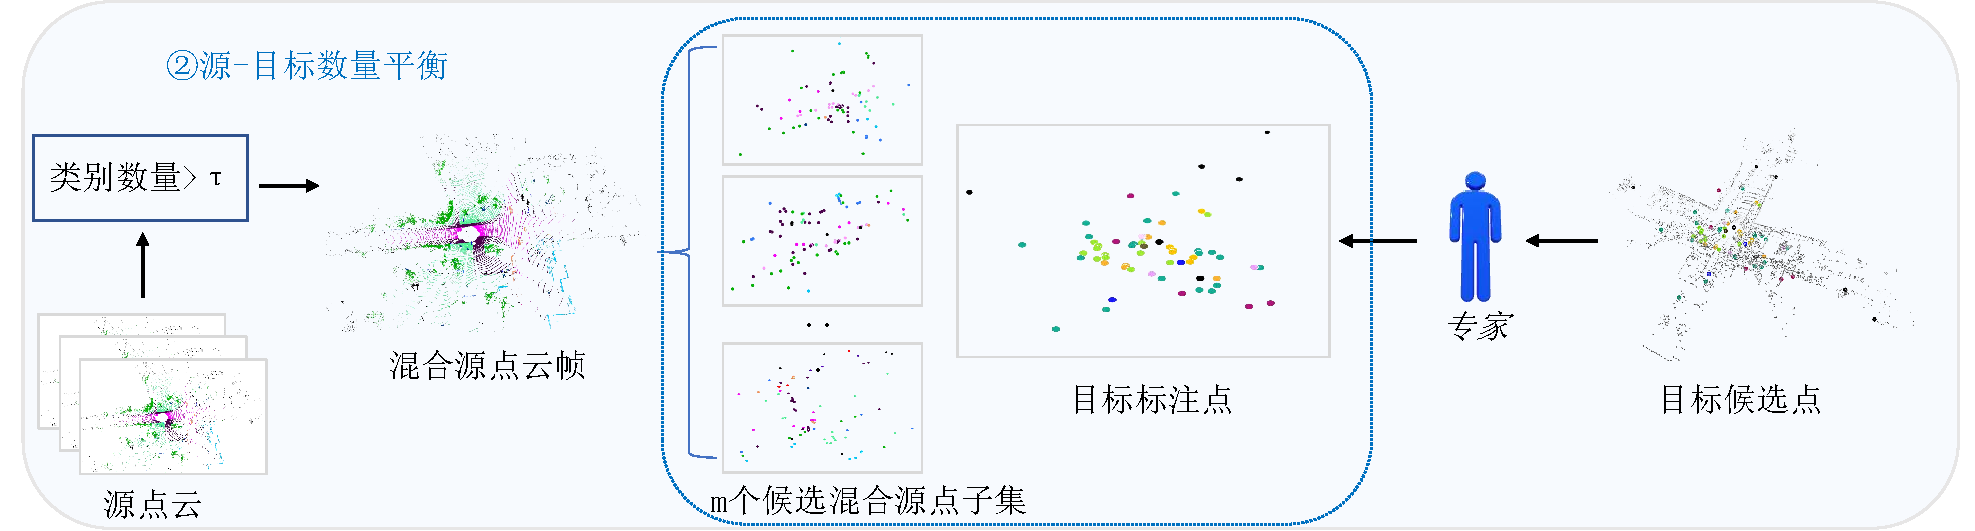
\includegraphics[width = \textwidth, scale=0.5]{ljx/figure/4-2s-t.pdf}
        \bicaption[\xiaosi 源-目标数量平衡模块]{\wuhao 源-目标数量平衡模块}{\wuhao Source-target amount balance module}
        \label{fig:4-2}
    \end{figure}
    \vspace{-0.35cm}
    \subsection{类别平衡主动混合算法}  %使用select的进行写吧,看一下那篇文章
    % 同上,可以参考SELECT,但是一定要注意的是把体素换成是我们的点云帧才行(1000个字左右)
    % 主动学习普遍存在的一个问题是类别不平衡问题,所选择的点是无法提前预知的,所有的策略都是基于模型进行推测的,因此目标域中每一帧点云各类别所含点的数量差异显著。而标注后的类别分布的结果后验于主动学习选择的结果,为了解决这个问题,在域适应任务中源域中拥有大量且标注的语义类别点,本章的方法就是选择一些语义分布更加均衡的源域点进行混合,这样既可以学习到域不变特征,又可以缓解类别不平衡的问题。
    % 主动学习普遍存在类别不平衡的问题。由于所选取的点无法提前预知,所有策略均基于模型推测,标注后的类别分布结果又依赖于主动学习的选择,这会导致目标域中每一帧点云各类别所含标注点数存在显著差异。而在域适应任务中,源域通常拥有大量带标注的语义类别点。因此,为解决这一问题,本章方法通过选择可以使得混合后类别分布更平衡的源域点,并使之与目标域标注点进行混合形成中间域数据并用于模型微调,这不仅有助于学习域不变特征,也能有效缓解类别不平衡的问题。
    针对主动学习在目标域中引发的类别不平衡问题,本章提出了类别平衡主动混合算法。在主动学习中,由于所选取点的类别无法提前预知,因此主动选择的点往往会导致目标域每一帧点云中各类别之间所含标注点数存在显著差异。值得关注的是,在跨域点云分割任务中,源域通常具备大量完整标注且可直接利用的语义类别点。而这为本章解决主动学习选择的类别不平衡提供了一个思路。如图\ref{fig:4-3}所示,从源域数据上选择候选点并与目标域标注点混合,使得混合后的数据中类别分布相对平衡。混合后的中间域数据不仅有助于学习域不变特征,也能有效缓解类别不平衡的问题。%。因此,本章方法通过选择可以使得混合后类别分布更平衡的源域点,并使之与目标域标注点进行混合形成中间域数据并用于模型微调,这不仅
    % 基于从源-目标数量平衡模块所得到的$m$个候选子集,本小节的平衡模块旨在从$\mathbf{Q}$中选取一个候选子集$\mathbf{q}_i$,使得其在所有被选中的候选子集中的类别分布最均衡。为此将根据混合后的点云集真实标签分布计算的熵作为选择的指标,以减轻标签不平衡。具体而言,训练集都是混合后的中间域数据,记$N_{all}$代表训练集中所有已标注的点数,$N_c$则为其中属于类别c的点的总数。而$N_{mix}$,$i$则代表候选子集$\mathbf{q}_i$与匹配的目标域标注点的的总点数,$N_{mix}^c$表示其中真实标签为类别c的点数。为确定是否应选择候选子集$\mathbf{q}_i$来实现更平衡的类别分布,通过将已选择的标注点总数$N_{all}$与当前选子集$\mathbf{q}_i$与匹配的目标域混合后的总点数相加,计算类别c的相对比例$\{R_{i,c}\}^C_{c=1}$,公式如\eqref{eq:class_rate}所示:

    基于源-目标数量平衡模块生成的$m$候选子集,平衡模块的核心任务是从集合$\mathbf{Q}$中选取最优子集$\mathbf{q}_{max}$,使得该子集与已选数据组合后的整体类别分布达到最优
    % \vspace{-0.1cm}
    \begin{figure}[h]
        \centering
        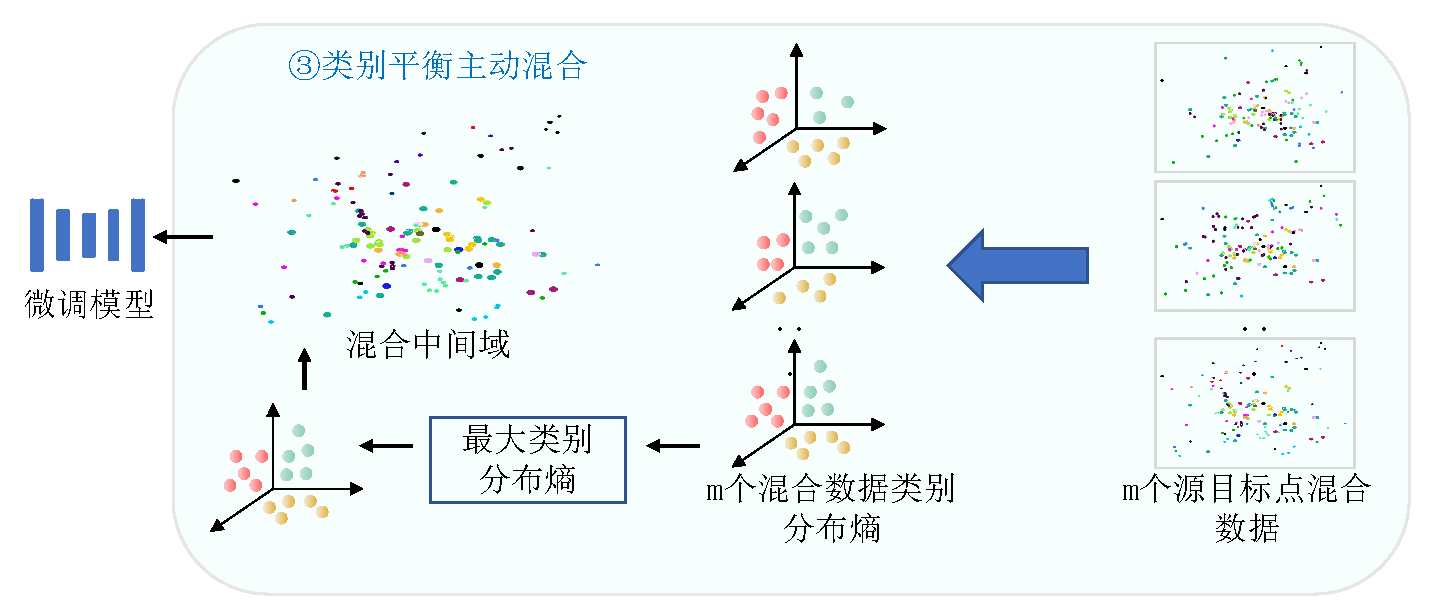
\includegraphics[width = \textwidth, scale=0.5]{ljx/figure/4-3am.pdf}
        \bicaption[\xiaosi 类别平衡主动混合模块]{\wuhao 类别平衡主动混合模块}{\wuhao Class-balanced active mixing module}
        \label{fig:4-3}
    \end{figure}
    % \vspace{-0.35cm}
    平衡状态。为实现这一目标,本模块采用信息熵作为量化指标,即通过计算候选子集与目标域数据混合后的真实标签分布熵值,筛选出能够最大程度缓解类别不平衡的候选子集。具体实施过程定义如下:设动态生成的中间域训练数据集包含$N_{all}$个已标注点,其中类别c的标注点数量为$N_c$。对于候选子集$\mathbf{q}_i$,其与对应目标域标注数据混合后形成的数据子集包含$N_{mix}$个点,其中类别的标注点数量为$N_{mix}^c$。为评估候选子集$\mathbf{q}_i$的平衡效果,需计算其引入后各类别的相对分布比例。具体方法是将已标注数据总量$N_{all}$与候选混合数据量$N_{mix}$进行叠加,按公式\eqref{eq:class_rate}逐类计算混合后的分布比例$\{R_{i,c}\}^C_{c=1}$。%最终通过后续的分布熵值比较实现最优子集选择。
    \begin{equation}
        \label{eq:class_rate}
        R_{i,c} = \frac{N_c+N^c_{mix}}{N_{all}+N_{mix}}
    \end{equation}
    同时,为了保证在同一个量纲下比较,对$R_{i,c}$使用softmax函数进行归一化处理,得到$\hat{R}_{i,c}$,如公式\eqref{eq:class_softmax}所示:
    \begin{equation}
        \label{eq:class_softmax}
        \hat{R}_{i,c}=\frac{e^{R_{i,c}}}{\sum^C_{c=1}e^{R_{i,c}}}
    \end{equation}
    其表示选择候选子集$\mathbf{q}_i$与当前已标注的目标点云帧混合后,各类别所占点数的归一化概率。再然后,通过计算分布的熵值来可作为候选子集的选择评判指标,如公式\eqref{eq:class_entropy}所示:
    \begin{equation}
        \label{eq:class_entropy}
        H_i(\hat{R}_{i})=-\sum_{c=1}^{C} \hat{R}_{i,c}\log(\hat{R}_{i,c})
    \end{equation}
    其中,$H_i$表示选择候选子集$\mathbf{q}_i$混合后类别分布的熵值结果,并选择熵值最大的一个候选子集$\mathbf{q}_{max}=\{\mathbf{X}_{\mathbf{q}_{max}},\mathbf{Y}_{\mathbf{q}_{max}}\}$作为最终混合源域集,与目标域标注点集$\mathbf{p}_i=\{\mathbf{X}_{p_i},\mathbf{Y}_{p_i}\}$组成新的中间域数据集$\mathbf{I}=\{\mathbf{\hat{X},\hat{Y}}\}$,如公式\eqref{eq:mix_final}所示:
    \begin{equation}
        \label{eq:mix_final}
        \begin{aligned}
            \mathbf{\hat{X}}=concat\{\mathbf{X}_{\mathbf{q}_{max}},\mathbf{X}_{\mathbf{p}_i}\}
            \\
        \mathbf{\hat{Y}}=concat\{\mathbf{Y}_{\mathbf{q}_{max}},\mathbf{Y}_{\mathbf{p}_i}\}
        \end{aligned}
    \end{equation}
    其中,$\mathbf{\hat{X}}$表示混合的点数据,$\mathbf{\hat{Y}}$则表示对应的标签。%将最终选择出的后选子集与目标域点进行混合,同时
    最后更新训练集总点数以及类别点数,公式如\eqref{eq:update_numeber}所示:
    \begin{equation}
        \label{eq:update_numeber}
        \begin{aligned}
            N_c=N_c+N^c_{mix}, \quad
            N_{all}=N_{all}+N_{mix}
        \end{aligned}
    \end{equation}
    
    \subsection{损失函数}
    % 对于后续的模型训练仅使用混合后的中间域数据进行微调训练,而混合后的数据都是含有标注的,因此本章使用交叉熵损失函数做为我们的优化损失函数,
    在后续的模型训练中,仅采用混合后的中间域数据进行微调优化。由于这些数据均包含标注信息,本章采用交叉熵损失函数作为优化策略,如公式\eqref{eq:cross_entropy}所示,其中$\hat{x}_{i} \in \hat{\mathbf{X}}$,$\hat{y}_{i} \in \hat{\mathbf{Y}}$:
    \begin{equation}
        \label{eq:cross_entropy}
        \mathcal{L}_{\text{CE}} = - \frac{1}{|I|} \sum_{i \in I} \sum_{c=1}^{C} \hat{y}_{i}^{c} \log h(\hat{x}_{i}^{c})
    \end{equation}

    \section{实验评估}
    \subsection{实验设置}
    在本章实验中,同样使用MinkowskiNet\upcite{MinkowskiNet}在Annotator中的PyTorch实现版本作为目标分割网络模型,并使用随机梯度下降(SGD)\upcite{SGD}作为学习优化器。所有实验都在单张NVIDIA RTX A6000 GPU上进行训练。本章方法同样在真实到真实以及合成到真实的跨域场景下分别进行了实验。对于所有的场景,主动学习全程总共执行5次迭代并达到预设标注预算。由于在四个跨域数据集上的映射类别数量不同,参数$\tau$在SynLiDAR$\to$SemanticKITTI、SynLiDAR$\to$SemanticPOSS、SemanticKITTI$\to$nuScenes和nuScenes$\to$SemanticKITTI分别设置为13、9、6、6,参数m统一设置为10。此外,对于其他实验参数的配置仍延续第三章的实验设定。
    \subsection{实验结果}
    本章方法同样在合成到真实场景下的跨域数据集SynLiDAR$\to$SemanticKITTI和SynLiDAR$\to$SemanticPOSS,以及真实到真实场景下的跨域数据集SemanticKITTI
    $\to$nuScenes和nuScenes$\to$SemanticKITTI上做了相应的实验,并与最先进的方法以及前一章的方法进行了对比以验证其有效性。为了公平比较,如果没有特殊标明标注预算的情况下,默认都是在0.1\%标注预算下做出的实验结果。
    \subsubsection{合成到真实场景}
    \begin{table}[H]
	\renewcommand{\arraystretch}{1}
    \centering
    \setlength{\tabcolsep}{10mm}
    \bicaption[\xiaosi 第三章方法与其他域适应方法在SynLiDAR\(\to\)SemanticKITTI数据上的比较]{\wuhao 本方法与其他域适应方法在SynLiDAR\(\to\)SemanticKITTI数据上的比较}{\wuhao Comparison with other domain adaptation methods on SynLiDAR\(\to\)SemanticKITTI}
    \label{tab:4-1}
    \wuhao
    \begin{tabular}{lccc}
        \toprule[1.5pt]
        \textbf{方法} & \textbf{域适应} & \textbf{标注} & \textbf{结果} \\
        \midrule
        Source-Only   & -          & -       & 22.8 \\
        Target-Only   & -          & 100\%       & 60.1 \\
        AADA          & UDA & -       & 23.0 \\
        AdvEnt        & UDA & -       & 25.8 \\
        CRST          & UDA & -       & 26.5 \\
        ST-PCt        & UDA & -       & 28.9 \\
        PolarMix      & UDA & -       & 32.2 \\
        CoSMix        & UDA & -       & 31.0 \\
        DGT-ST        & UDA & -       & 43.1 \\
        MME           & SSDA & 0.04\%  & 24.5 \\
        APE           & SSDA & 0.04\%  & 25.1 \\
        APE-PCT       & SSDA & 0.04\%  & 27.0 \\
        CoSMix-SSDA   & SSDA & 0.04\%  & 34.3 \\
        本章方法       & SSDA   & 0.04\%   & 50.5 \\
        Annotator     & ADA   & 0.1\%     & 57.7 \\
        前章方法     & ADA   & 0.1\%     & 58.7 \\
        \textbf{本章方法}       & ADA   & 0.1\%     & \textbf{65.5} \\
        \bottomrule[1.5pt]
    \end{tabular}
\end{table}
    本章在SynLiDAR$\to$SemanticKITTI跨域数据集上的实验如表\ref{tab:4-1}所示,分析对比不同的结果可知,在没有任何域适应的情况下,Source-Only模型在目标域上的性能非常低,仅有22.8\%,这说明直接将源域训练的模型用到目标域效果很差。而使用全部目标域数据训练的模型(Target-Only)达到了60.1\%的结果,这说明域间隙的存在会导致在源域训练好的模型在目标域上性能急剧下降。
    % 说明目标域本身的标注数据确实能极大提升效果,但现实中很难获取这么多标注数据。因此需要研究如何在标注有限的情况下提升性能。

    在不需要目标域标注的无监督域适应(UDA)方法中,DGT-ST的效果最好,达到43.1\%,比Source-Only提升了近20个百分点,但相比Target-Only仍有较大差距。这说明即使不标注目标域数据,通过域适应也能部分缩小域间差异,但还不能完全解决问题。
    为了与半监督域适应方法进行公平比较,本章将主动学习的标注预算降低到与半监督同一量级即0.04\%,即使在这种极少量的标注下,本章方法仍达到了50.5\%的结果,比同样标注量的CoSMix-SSDA高出了近16个百分点。这说明在标注极少的情况下,本章方法能更有效地利用有限的标注信息。

    在与主动域适应方法进行比较时,标注比例提升到0.1\%,本章方法的结果达到了65.5\%,不仅比前章方法提高了近7个百分点,甚至超越了Target-Only,这说明本章方法构建的中间域增强了模型的性能,学习到了源和目标域的信息,因此超越了全监督结果。当然,超越Target-Only本算法并非先例,在之前的一些域适应文章中\upcite{schachtsiek2023classf}也有做到。另外,值得注意的是,虽然标注量增加了2.5倍,但性能提升幅度远高于标注量的增长比例,这说明在前一章的基础上,结合本章主动混合策略,充分发挥了它们的最佳性能。
    % 能够充分发挥二者的深度结合优势。
    % 本章主动混合策略结合前一章源域指导的主动学习方法,能够充分发挥了其最佳性能。
    
    % \begin{table}[htbp]
\begin{table}[H]
	\renewcommand{\arraystretch}{1}
    \centering
    \setlength{\tabcolsep}{10mm}
    \bicaption[\xiaosi 第四章方法与其他域适应方法在SynLiDAR\(\to\)SemanticPOSS数据上的比较]{\wuhao 本章方法与其他域适应方法在SynLiDAR\(\to\)SemanticPOSS数据上的比较}{\wuhao Comparison with other domain adaptation methods on SynLiDAR\(\to\)SemanticPOSS}
    \label{tab:4-2}
    \wuhao
    \begin{tabular}{cccc}
        \toprule[1.5pt]
        \textbf{方法} & \textbf{域适应} & \textbf{标注} & \textbf{结果} \\
        \midrule
        Source-Only   & -           & -       & 34.6 \\
        Target-Only   & -           & 100\%       & 58.0 \\
        CRST\upcite{zou2019confidence}          & UDA & -       & 27.1 \\
        ST-PCT\upcite{xiao2022transfer}        & UDA & -       & 29.6 \\
        PolarMix\upcite{xiao2022polarmix}      & UDA & -       & 30.4 \\
        CoSMix\upcite{saltori2022cosmix}        & UDA & -       & 40.4 \\
        DGT-ST\upcite{yuan2024density}        & UDA & -       & 50.8 \\
        MME\upcite{saito2019semi}           & SSDA & 0.01\%  & 33.2 \\
        APE\upcite{APE}           & SSDA & 0.01\%  & 30.3 \\
        APE-PCT\upcite{xiao2022transfer}       & SSDA & 0.01\%  & 31.2 \\
        CoSMix-SSDA\upcite{saltori2023compositional}   & SSDA & 0.01\%  & 41.0 \\
        本章方法       & SSDA   & 0.01\%   & 57.5 \\
        Annotator\upcite{Annotator}     & ADA   & 0.1\%     & 52.0 \\
        前章方法       & SSDA   & 0.1\%   & 56.6 \\
        \textbf{本章方法}       & ADA   & 0.1\%     & \textbf{60.2} \\
        \bottomrule[1.5pt]
    \end{tabular}
\end{table}
    如表\ref{tab:4-2}结果显示,在SynLiDAR$\to$SemanticPOSS数据集上域差异依然显著。在无监督域适应(UDA)中,DGT-ST以50.8\%的表现达到最优,但距离全标注仍有7个百分点的差距。本章方法在0.01\%的极低标注预算下达到了57.5\%的结果,远超CoSMix-SSDA,甚至接近Target-Only水平。当与主动域适应方法(ADA)进行比较时,标注量提升至0.1\%,本章方法以60.2\%的结果超越前章方法和Annotator分别3.6和7.8个百分点,超过Targe-Only2.2个百分点,这证明本章的主动混合策略是有效果的,在结合第三章的方法后可以大幅度提升模型性能。
    % 最后,提供了合成到真实场景下的可视化结果,以真实标签为参照,与前章方法进行对比,以证明本章方法的有效性,可视化结果如图\ref{fig:4-5}所示:
    % \vspace{-0.1cm}
    % \begin{figure}[h]
    %     \centering
    %     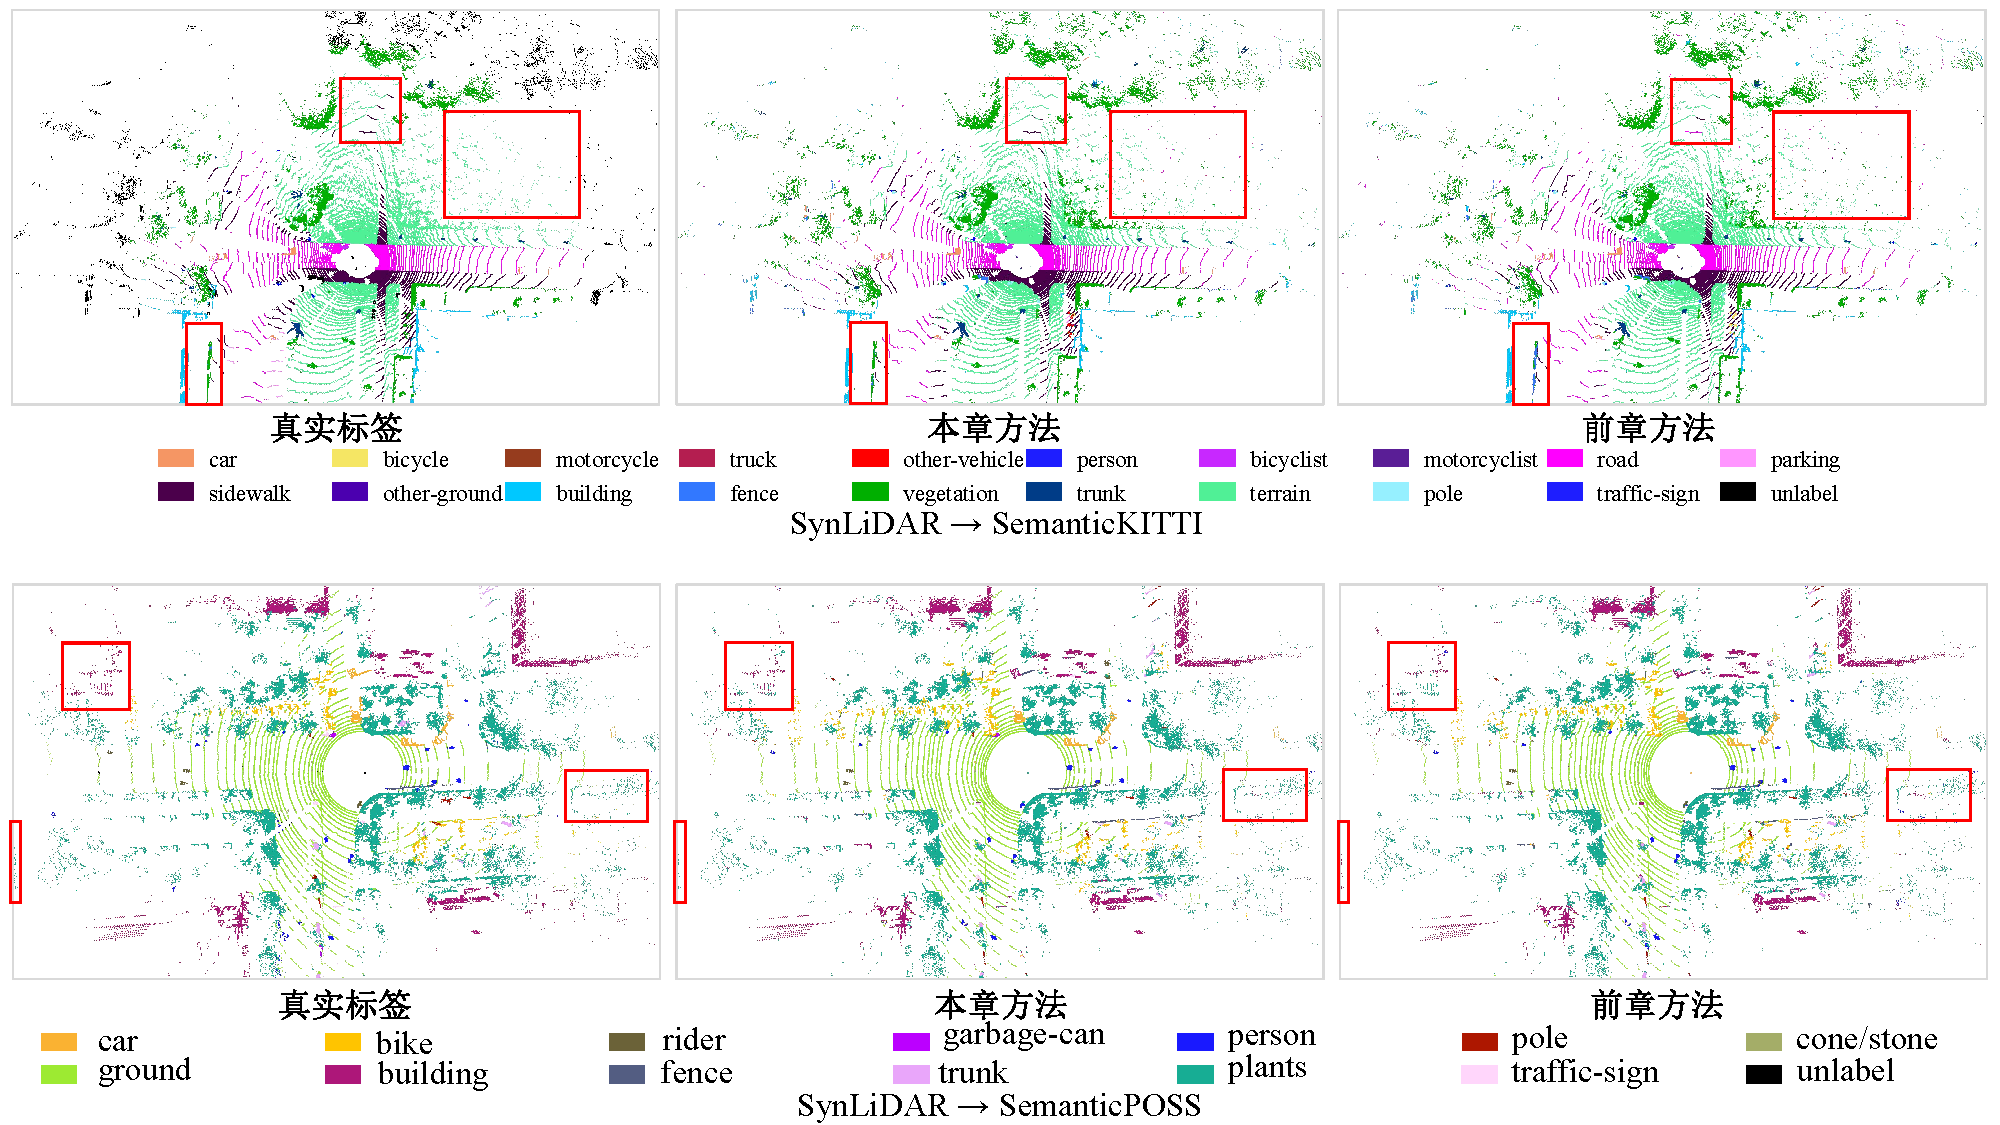
\includegraphics[width = \textwidth, scale=0.5]{ljx/figure/4-5s2r.pdf}
    %     \bicaption[\xiaosi 类别平衡主动混合模块]{\wuhao 类别平衡主动混合模块}{\wuhao Class-balanced active mixing module}
    %     \label{fig:4-5}
    % \end{figure}
    % \vspace{-0.35cm}
    % 证明第三章所提出的主动学习筛选能大幅降低标注成本选择对域适应最有帮助的域差异点,同时也证明本章的主动混合策略可以大幅提升其效果。
    % 通过表4-2的数据对比,可以看出不同域适应方法在SynLiDAR→SemanticPOSS数据集上的表现差异。从Source-Only(34.6)和Target-Only(58.0)的对比来看,两个领域的差异依然显著,直接迁移源域模型的效果有限,而完全标注目标域虽能大幅提升性能,但实际应用中标注成本过高的问题依然存在。  
    % 在无监督域适应(UDA)方法中,DGT-ST的表现最好,达到了50.8,远高于其他UDA方法(如CRST的27.1、CoSMix的40.4)。这说明DGT-ST在无标注情况下能较好地缓解域差异,但距离Target-Only仍有7分左右的差距,表明无监督方法在复杂场景中仍有优化空间。  
    % 当标注量仅为0.01\%(SSDA场景)时,本章方法以57.5的得分远超其他SSDA方法。例如,CoSMix-SSDA仅达到41.0,而本章方法比其高出16.5分,甚至接近Target-Only的58.0。这表明即使标注量极少,通过动态筛选源域数据并与目标域混合的策略,能更有效地利用有限标注信息,显著缩小域间差距。值得注意的是,本章方法的SSDA结果(57.5)甚至超过了部分标注量更高的ADA方法(如Annotator的52.0),进一步验证了该策略的高效性。  
    % 当标注量提升到0.1\%(ADA场景)时,本章方法得分60.2,不仅比前章方法(56.6)提高了3.6分,还超过了Annotator的52.0。虽然标注量增加了10倍(从0.01\%到0.1\%),但性能提升幅度(从57.5到60.2)相对较小,可能说明在极低标注量下模型性能已接近上限,或需要更精细的样本选择策略。此外,本章方法在ADA场景下的结果(60.2)与Target-Only(58.0)的差距缩小到仅2.2分,这表明通过主动学习筛选高价值样本,能在少量标注下实现接近全标注的效果,大幅降低实际应用成本。  

    % 整体来看,本章方法在两种标注场景下均展现出较强优势,尤其是在极低标注量(0.01\%)时,其性能已接近部分高标注量方法的结果,验证了动态混合策略在跨域数据平衡中的重要性。
    \subsubsection{真实到真实场景}
    SemanticKITTI$\to$nuScenes的结果如表\ref{tab:4-3}所示,Source-Only模型在目标域的结果仅为33.7\%,而全标注的Target-Only模型则达到了82.7\%,这验证了真实到真实跨域场景中源域与目标域的巨大差异。在无监督域适应(UDA)方法中,LiDOG以34.9\%的表现最优,但仍远低于全标注结果,表明纯无监督策略在复杂域差异下的局限性。在主动域适应(ADA)场景下,本章方法以81.0\%的结果显著超越Annotator的75.9\%,提升幅度达5.1分,且与Target-Only的差距缩小至1.7个百分点,同时与前章方法相比,提升了4.5个百分点。从上述实验结果可知本章方法通过主动混合策略有效利用有限标注信息与源域数据,在极低标注成本下逼近全标注性能,证明了其在真实跨域场景中的有效性。
    % \begin{table}[htbp]
\begin{table}[H]
	\renewcommand{\arraystretch}{1}
    \centering
    \setlength{\tabcolsep}{12mm}
    \bicaption[\xiaosi 第四章方法与其他域适应方法在SemanticKITTI\(\to\)nuScenes数据上的比较]{\wuhao 本章方法与其他域适应方法在SemanticKITTI\(\to\)nuScenes数据上的比较}{\wuhao Comparison with other domain adaptation methods on SemanticKITTI\(\to\)nuScenes}
    \label{tab:4-3}
    \wuhao
    \begin{tabular}{cccc}
        \toprule[1.5pt]
        \textbf{方法} & \textbf{域适应} & \textbf{标注} & \textbf{mIoU(\%)} \\
        \midrule
        Source-Only   & -       & -           & 33.7 \\
        Target-Only   & -       & 100\%           & 82.7 \\
        Mix3D\upcite{nekrasov2021mix3d}         & UDA     & -   & 31.5 \\
        CoSMix\upcite{saltori2022cosmix}        & UDA     & -   & 29.8 \\
        SN\upcite{wang2020train}              & UDA   & -     & 25.8 \\
        RayCast\upcite{langer2020domain}        & UDA    & -    & 30.9 \\
        LiDOG\upcite{saltori2023walking}        & UDA      & -       & 34.9 \\
        前章方法       & ADA    & 0.1\%      & 76.5 \\
        Annotator\upcite{Annotator}     & ADA     & 0.1\%     & 75.9 \\
        \textbf{本章方法}       & ADA    & 0.1\%      & \textbf{81.0} \\
        \bottomrule[1.5pt]
    \end{tabular}
\end{table}
    如表\ref{tab:4-4}数据显示,在nuScenes$\to$SemanticKITTI的实验结果中,Source-Only模型仅得32.5\%,而Target-Only模型通过全标注数据达到85.4\%,再次印证域差异的显著影响。在无监督域适应(UDA)方法中,LiDOG以41.2\%的表现依然取得最优,但仍与全标注结果相差44.2个百分点。在标注量仅0.1\%的主动域适应(ADA)场景下,本章方法以86.2\%的结果超越目标域全监督(Target-Only)0.8个百分点,远超Annotator的81.8\%,超越前章方法3.2个百分点。本章方法的突破性结果表明,通过主动混合策略在极低标注量下超越了全标注的性能,进一步证明了本章方法的真实有效性。
    % 大幅降低了实际应用中对标注数据的依赖。这一结果进一步验证了源-目标协同优化策略在跨域任务中的高效性。
    % \begin{table}[htbp]
\begin{table}[H]
	\renewcommand{\arraystretch}{1}
    \centering
    \setlength{\tabcolsep}{12mm}
    \bicaption[\xiaosi 第四章方法与其他域适应方法在nuScenes\(\to\)SemanticKITTI数据上的比较]{\wuhao 本章方法与其他域适应方法在nuScenes\(\to\)SemanticKITTI数据上的比较}{\wuhao Comparison with other domain adaptation methods on nuScenes\(\to\)SemanticKITTI}
    \label{tab:4-4}
    \wuhao
    \begin{tabular}{cccc}
        \toprule[1.5pt]
        \textbf{方法} & \textbf{域适应} & \textbf{标注} & \textbf{mIoU(\%)} \\
        \midrule
        Source-Only   & -       & -           & 32.5 \\
        Target-Only   & -       & 100\%           & 85.4 \\
        Mix3D\upcite{nekrasov2021mix3d}         & UDA    & -   & 32.4 \\
        CoSMix\upcite{saltori2022cosmix}        & UDA     & -   & 36.8 \\
        SN\upcite{wang2020train}              & UDA   & -     & 23.6 \\
        RayCast\upcite{langer2020domain}        & UDA    & -    & 31.5 \\
        LiDOG\upcite{saltori2023walking}        & UDA      & -       & 41.2 \\
        前章方法       & ADA    & 0.1\%      & 83.0 \\
        Annotator\upcite{Annotator}     & ADA     & 0.1\%     & 81.8 \\
        \textbf{本章方法}       & ADA    & 0.1\%      & \textbf{86.2} \\
        \bottomrule[1.5pt]
    \end{tabular}
\end{table}
    \subsubsection{分割可视化结果}
    \vspace{-0.1cm}
    \begin{figure}[h]
        \centering
        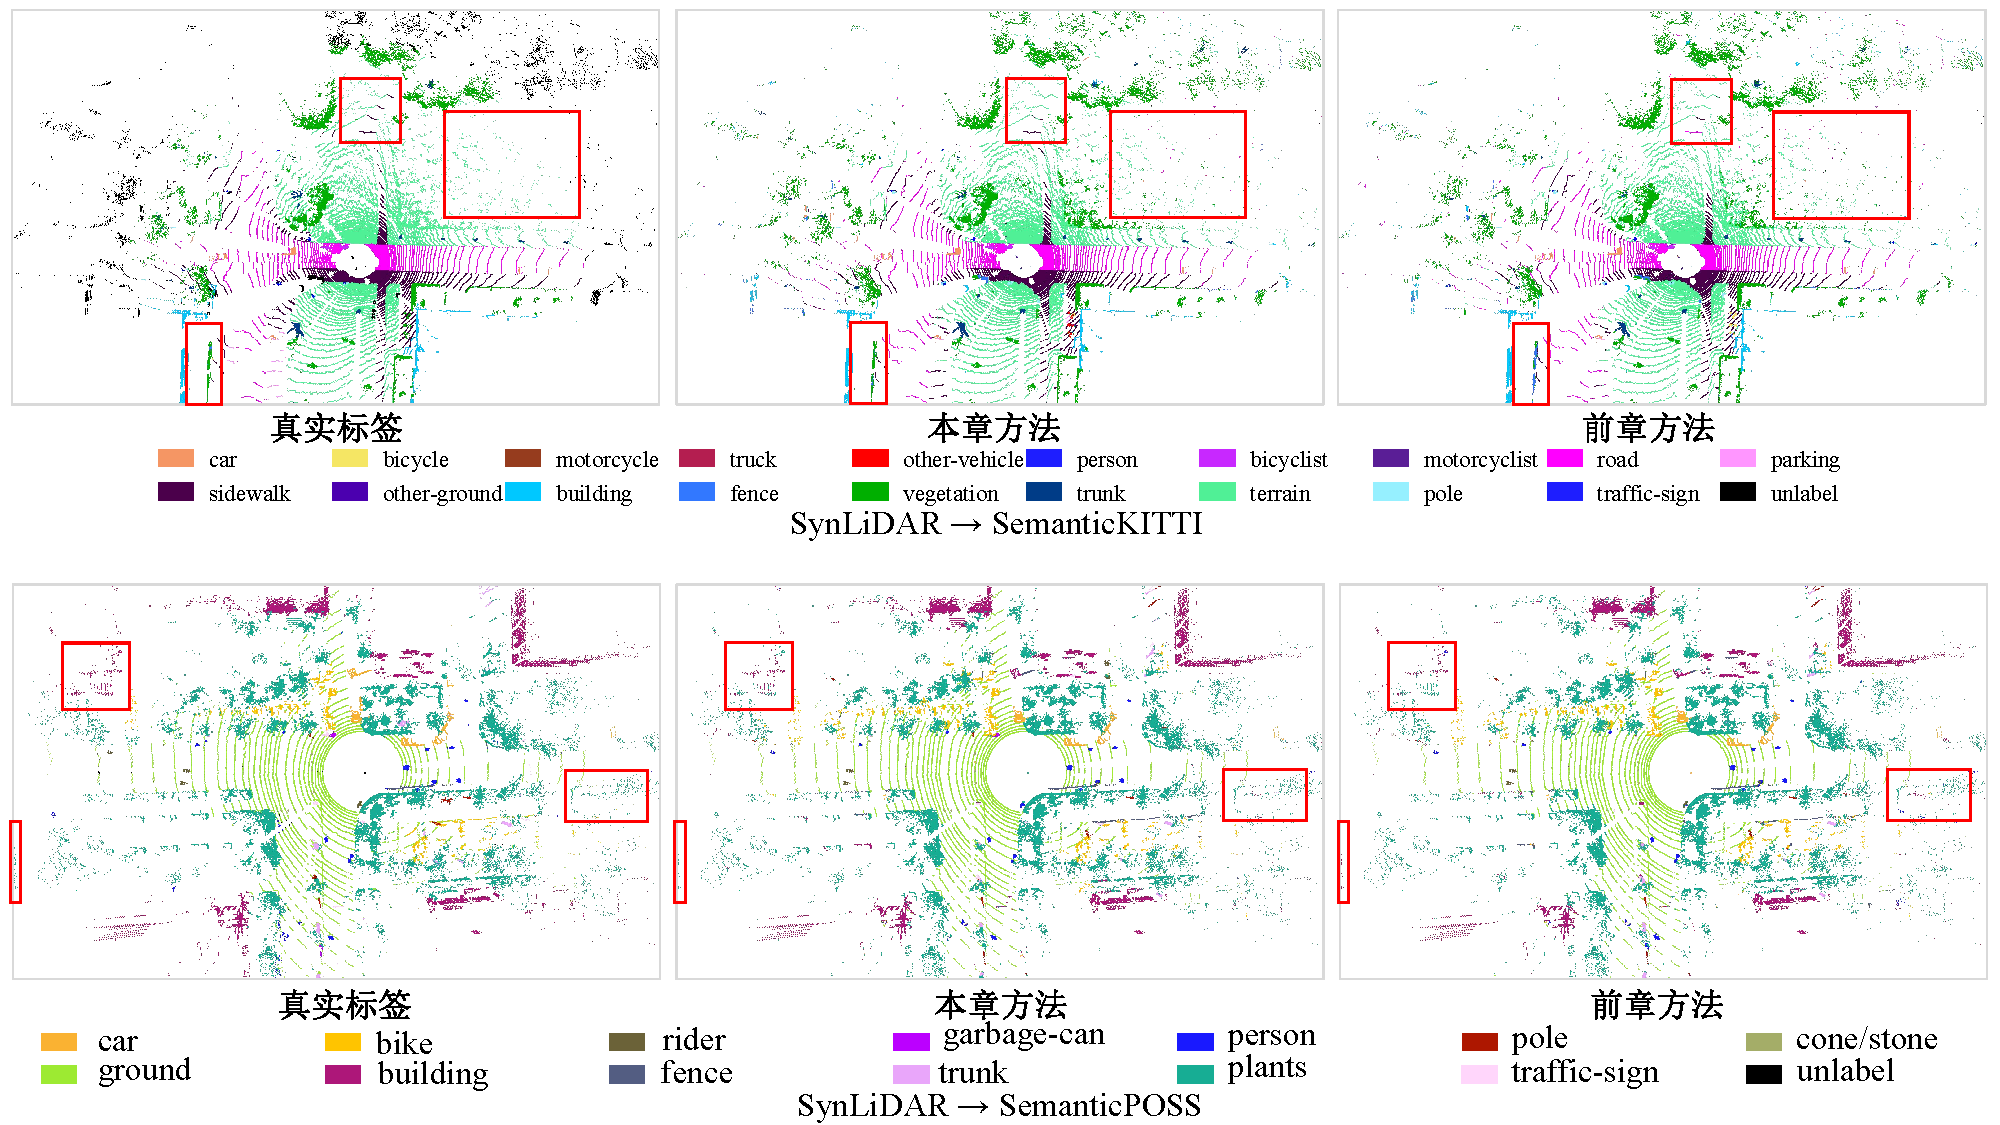
\includegraphics[width = \textwidth, scale=0.5]{ljx/figure/4-5s2r.pdf}
        \bicaption[\xiaosi 第四章方法在合成到真实场景分割可视化图]{\wuhao 本章方法在合成到真实场景分割可视化图}{\wuhao Visualization of the segmentation results in the synthetic-to-real}
        \label{fig:4-5}
    \end{figure}
    \vspace{-0.35cm}
    为了进一步证明本章方法的有效性,提供了合成到真实场景下的可视化结果如图\ref{fig:4-5}所示。以真实标签为参照,与前章方法进行对比,使用红框标出差异区域,可以看到本章方法在一些语义边界处有着更好的辨别效果。同样的,本章也提供了真实到真实场景下的可视化结果如图\ref{fig:4-6}所示。本章方法在人造物品、人行道等边缘类别取得了更好的 分割效果。
    \vspace{-0.1cm}
    \begin{figure}[h]
        \centering
        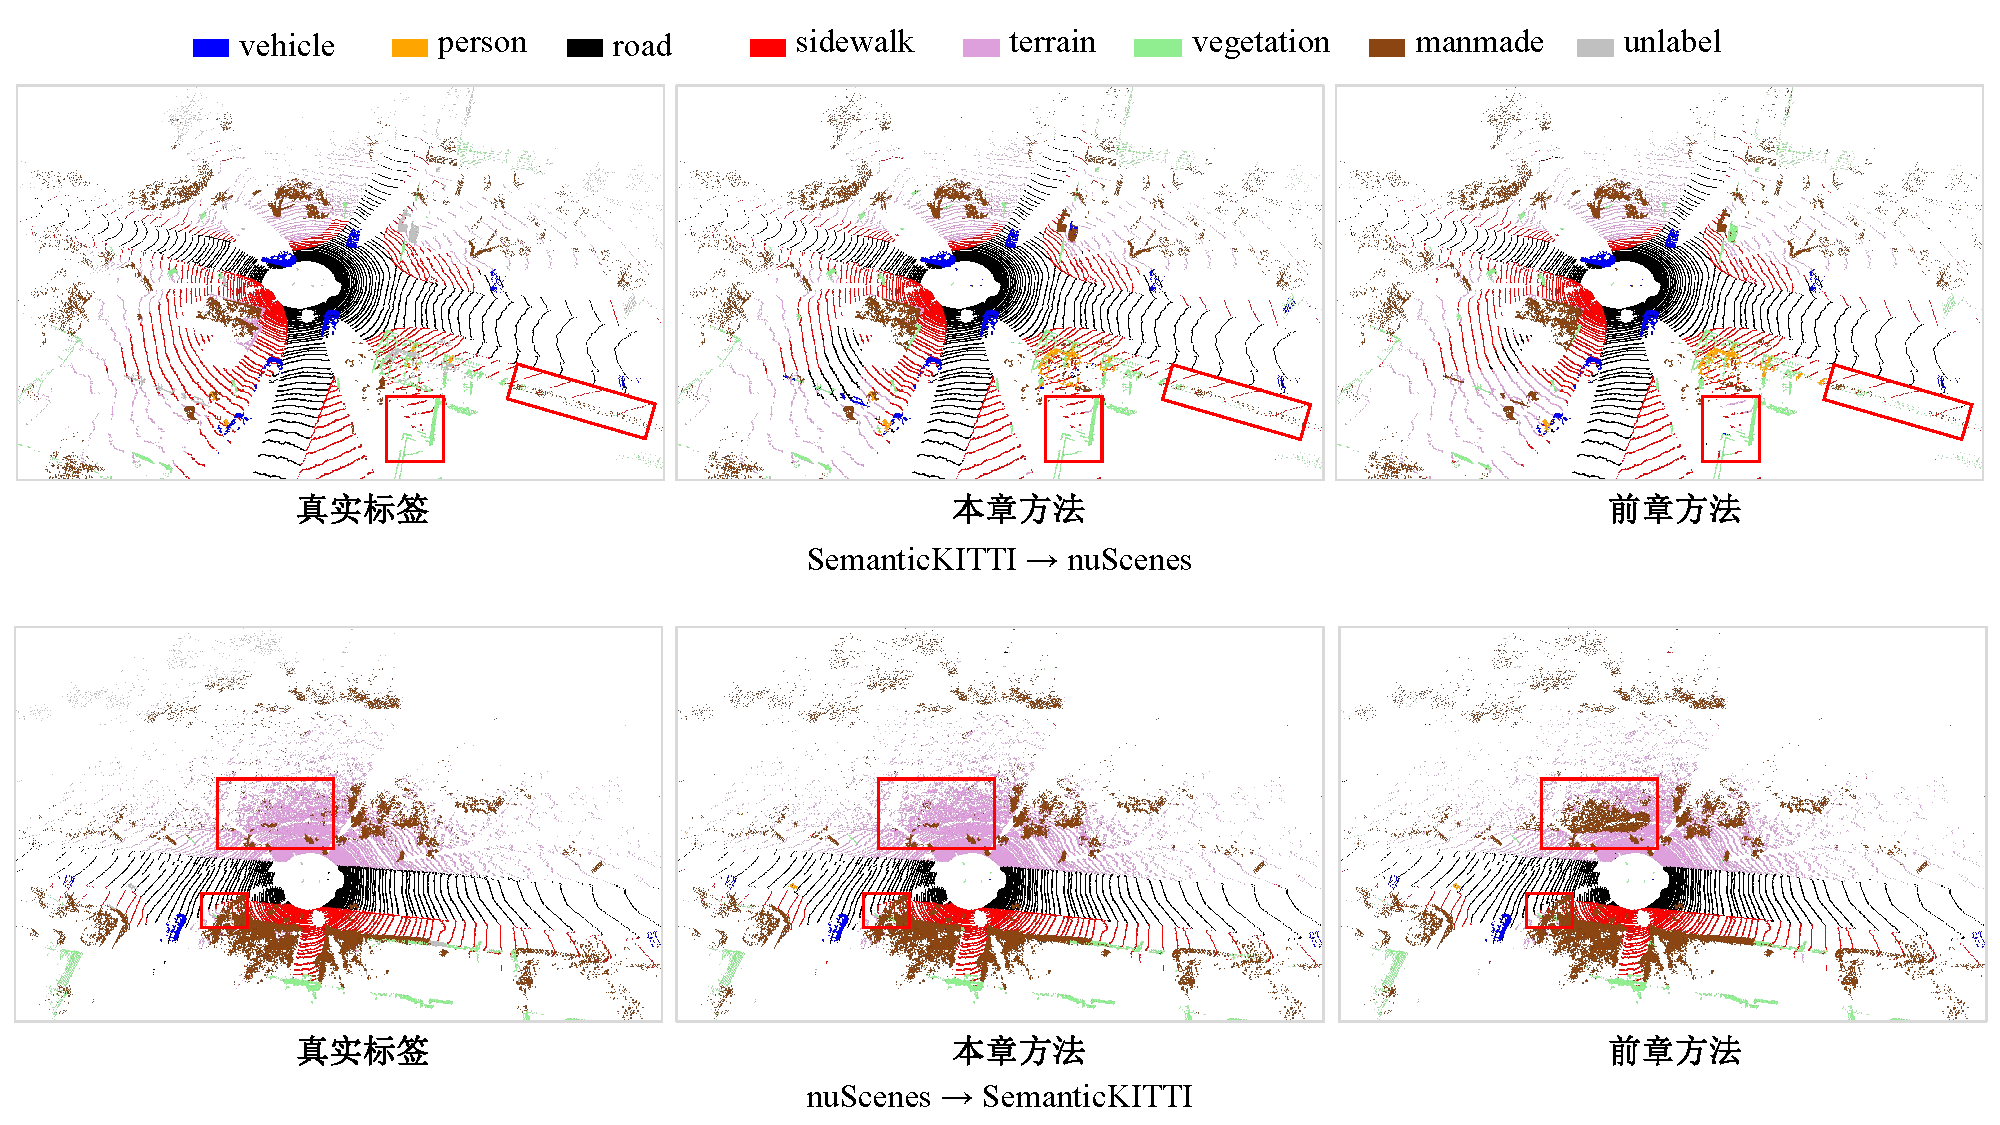
\includegraphics[width = \textwidth, scale=0.5]{ljx/figure/4-6r2r.pdf}
        \bicaption[\xiaosi 第四章方法在真实到真实场景分割可视化图]{\wuhao 本章方法在真实到真实场景分割可视化图}{\wuhao Visualization of the segmentation results in the real-to-real}
        \label{fig:4-6}
    \end{figure}
    \vspace{-0.35cm}
    \subsection{消融对比实验}
    % 把所有的能放的图和表全放上来
    \subsubsection{对比实验}
    \begin{table}[H]
	\renewcommand{\arraystretch}{1}
    \centering
    \setlength{\tabcolsep}{10mm}
    \bicaption[\xiaosi 第四章方法与其他Mixing方法在SynLiDAR$\to$SemanticKITTI数据上的比较]{\wuhao 本章方法与其他Mixing方法在SynLiDAR$\to$SemanticKITTI数据上的比较}{\wuhao Comparison with other mixing methods on SynLiDAR$\to$SemanticKITTI}
    \label{tab:4-6}
    \wuhao
    \begin{tabular}{cccc}
        \toprule[1.5pt]
        \textbf{主动学习} & \textbf{Mixing方法} & \textbf{标注} & \textbf{结果} \\
        \midrule
        \multirow{3}{*}{SPAL} & LaserMix\upcite{kong2023lasermix} & 0.1\% & 39.6 \\
        ~& PolarMix\upcite{xiao2022polarmix} & 0.1\% & 46.6 \\
        ~& \textbf{Ours} & 0.1\% & \textbf{65.5} \\
        \bottomrule[1.5pt]
    \end{tabular}
\end{table}
    为证明本章方法的有效性,在SynLiDAR$\to$SemanticKITTI上进行了与其他传统Mixing方法的对比实验,在SPAL框架下统一采用0.1\%标注量进行公平比较,实验结果如表\ref{tab:4-6}所示。实验中,PolarMix和LaerMix都是按照1/4比例进行混合,即源和目标交换自身1/4圆周角度内的点或者1/4线束角度内的点进行混合。在相同标注条件下,LaserMix和PolarMix方法分别取得39.6\%和46.6\%的性能结果,而本章提出的方法以65.5\%的显著优势超越了它们,性能提升幅度达25.9\%和18.9\%。这一结果验证了传统混合方法在跨域数据融合时对类别分布不敏感,数量过多导致模型学习的知识更偏向源域等问题,而本章方法通过源-目标的数量平衡算法以及熵驱动的源域筛选机制与动态平衡算法,能够精准选择与目标域互补的源域样本,有效缓解混合过程中的类别不均衡问题。%因此,基于固定几何变换的混合策略通常难以适应复杂域差异场景,本章方法在相同标注约束下的突破性表现,进一步证明了基于点云语义分割域适应的主动混合策略在跨域主动学习中价值。
    \vspace{-0.1cm}
    \begin{figure}[H]
        \centering
        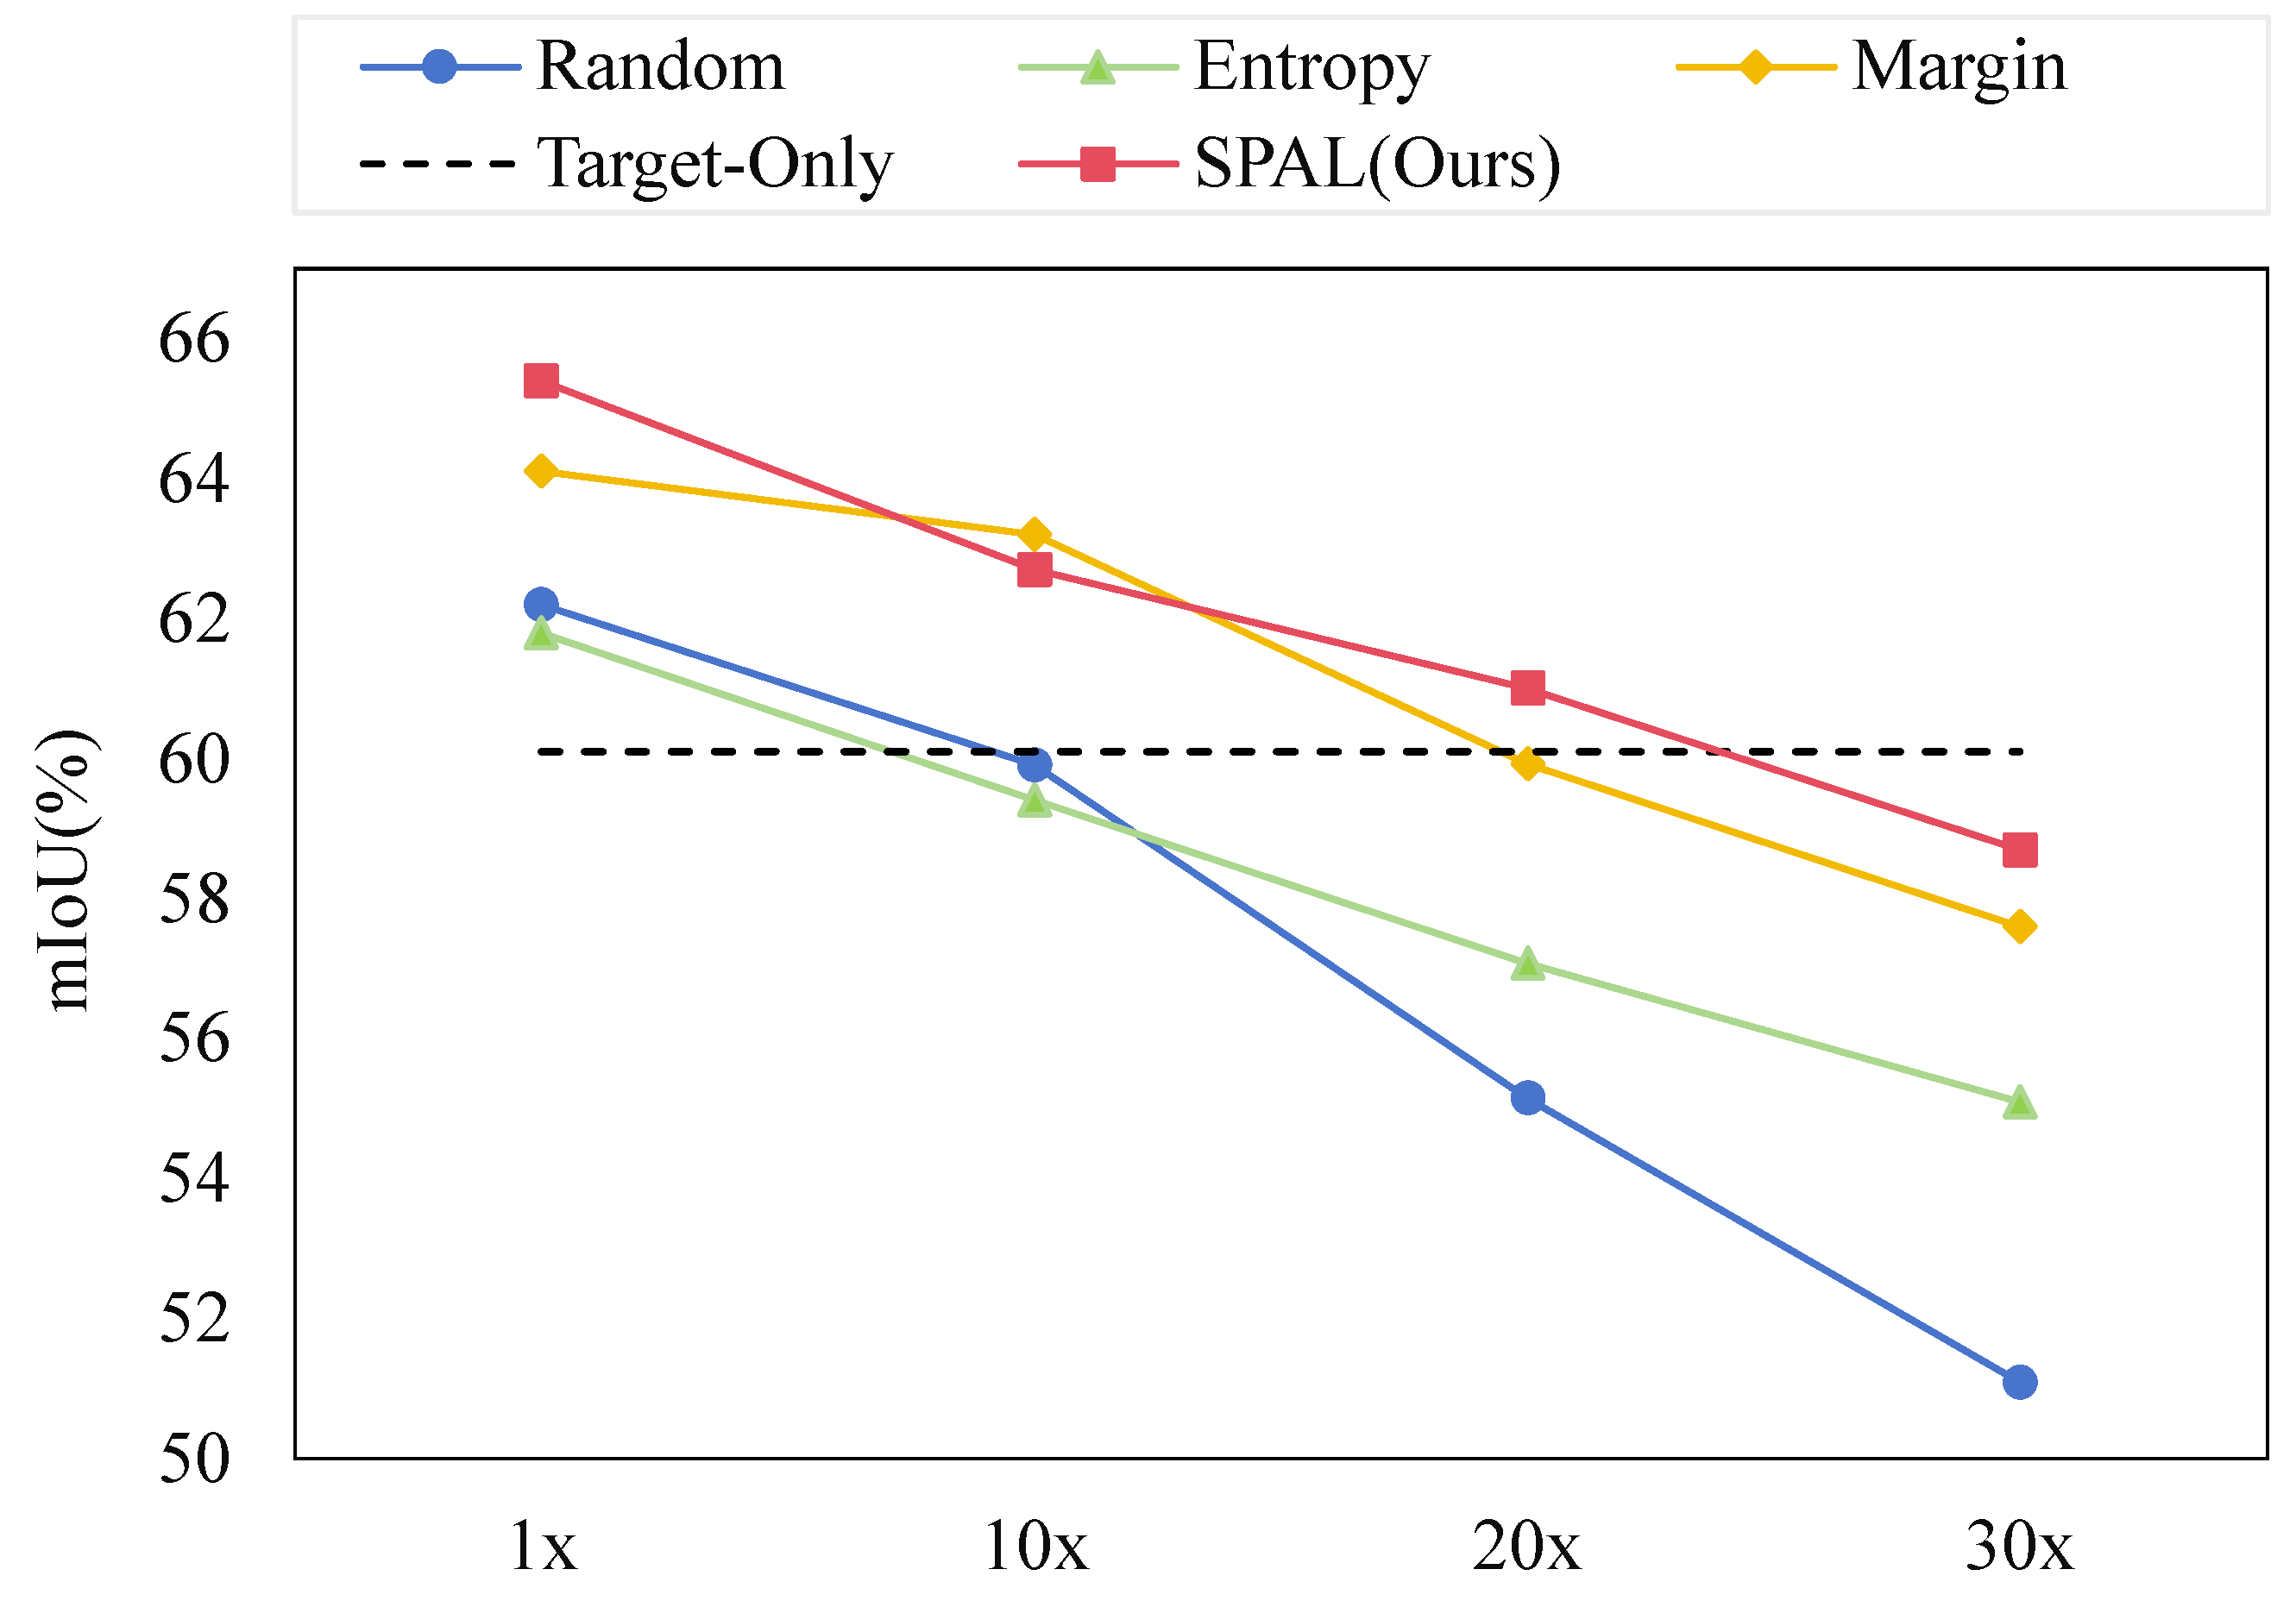
\includegraphics[width = \textwidth]{ljx/figure/4-compare-al-mixing.pdf}
        \bicaption[\xiaosi 第四章方法结合不同主动学习在多个混合比例下的对比结果]{\wuhao 本章方法结合不同主动学习在多个混合比例下的对比结果}{\wuhao Comparison results of different active learning methods under various mixing ratios}
        \label{fig:4-compare-al-mixing}
    \end{figure}
    \vspace{-0.35cm}
    如图\ref{fig:4-compare-al-mixing}所示,本章在SynLiDAR$\to$SemanticKITTI数据集上进行了对比实验,展示了不同主动学习策略在不同源-目标混合比例下的性能对比。其中,1x代表的是本章提出的源-目标域数量平衡算法(即源域与目标域数据按1:1比例动态混合),10x代表源域与目标域数据按10:1比例动态混合,20x和30x则分别代表源域与目标域数据按20:1和30:1比例进行动态混合。实验结果显示,在默认0.1\%的标注预算下,本章混合方法在多种主动学习方法中均取得了最优的结果,这证明了算法的有效性,根据域适应以及主动学习的特点,简单高效的提升了性能。而在源-目标域数量平衡算法下,前一章提出的SPAL方法的结果又是最高的,达到了65.5\%的结果,这证明了SPAL与本章方法结合的有效性。
    
    为证明本章方法结合前章SPAL方法的的有效性,在四个跨域数据集(SynLiDAR$\to$SemanticKITTI、
    SynLiDAR$\to$SemanticPOSS、SemanticKITTI$\to$nuScenes、nuSc-
    enes$\to$SemanticKITTI)上均进行了实验。如表\ref{tab:4-5}所示,在四个跨域数据实验中,结合两章的算法均取得最高结果,且稳定超越其他主动学习方法。这验证了第四章提出的主动混合策略与第三章SPAL框架结合的有效性和普适性。这一跨数据集的全面优势表明,源-目标平衡机制能够适配不同域差异场景,显著提升模型的性能。
    % 换成竖的
% \begin{table}[ht]%[t]
%     \centering
%     \resizebox{\linewidth}{!}
%     {
%         \large
%         \begin{tabular}{@{}l|c|c@{}}
%             \toprule
%             Methods & SynLiDAR $\to$ SemanticKITTI & SynLiDAR $\to$ SemanticPOSS \\
%             \midrule
%             Source-/Target-Only & 22.0 / 61.1 & 34.5 / 57.9 \\
%             % \midrule
%             Random & 62.2 & 58.3 \\
%             Entropy & 61.8 & 55.6 \\
%             Margin & 64.0 & 60.0 \\
%             \revision{VCD}~\cite{xie2023annotator} & 56.8 & 45.5 \\
%             \textbf{SPAL (Ours)} & \revision{\textbf{65.5}} & \textbf{60.2} \\
%             \bottomrule 
%         \end{tabular}
%     }
%     \caption{Comparison of different active query strategies for domain adaptation on MinkNet~\cite{choy20194d} with a 0.1\% budget and a mixing rate of $1$x. Our query strategy consistently achieves superior performance both SynLiDAR $\to$ SemanticKITTI and SynLiDAR $\to$ SemanticPOSS.}
%     \label{tab:active_query}
% \end{table}

% \begin{table}[htbp]
\begin{table}[H]
    \vspace{-0.05cm}
	\renewcommand{\arraystretch}{1}
    \centering
    \setlength{\tabcolsep}{10mm}
    \bicaption[\xiaosi 第四章方法结合不同主动学习方法结果对比]{\wuhao 本章方法结合不同主动学习方法结果对比}{\wuhao  Comparison with different active learning methods that incorporate this chapter's modules}
    \label{tab:4-5}
    \wuhao
    \begin{tabular}{cccc}
        \toprule[1.5pt]
        \textbf{数据集} & \textbf{方法} & \textbf{标注} & \textbf{mIoU(\%)} \\
        \midrule
        \multirow{4}{*}{SynLiDAR\(\to\)SemanticKITTI} & 
        Random              & 0.1\%        & 62.2 \\
        ~ & Entropy\upcite{Entropy}             & 0.1\%        & 61.8 \\
        ~ & Margin\upcite{Margin}              & 0.1\%        & 64.0 \\
        ~ & \textbf{SPAL}          & 0.1\%        & \textbf{65.5} \\
        \multirow{4}{*}{SynLiDAR\(\to\)SemanticPOSS} & 
        Random              & 0.1\%        & 58.3 \\
        ~ & Entropy\upcite{Entropy}             & 0.1\%        & 55.6 \\
        ~ & Margin\upcite{Margin}              & 0.1\%        & 60.0 \\
        ~ & \textbf{SPAL}          & 0.1\%        & \textbf{60.2} \\
        \multirow{4}{*}{SemanticKITTI\(\to\)nuScenes} & 
        Random              & 0.1\%        & 85.7 \\
        ~ & Entropy\upcite{Entropy}             & 0.1\%        & 83.2 \\
        ~ & Margin\upcite{Margin}              & 0.1\%        & 85.9 \\
        ~ & \textbf{SPAL}          & 0.1\%        & \textbf{86.2} \\
        \multirow{4}{*}{nuScenes\(\to\)SemanticKITTI} & 
        Random              & 0.1\%        & 77.7 \\
        ~ & Entropy\upcite{Entropy}             & 0.1\%        & 76.5 \\
        ~ & Margin\upcite{Margin}              & 0.1\%        & 80.7 \\
        ~ & \textbf{SPAL}          & 0.1\%        & \textbf{81.0} \\
        \bottomrule[1.5pt]
    \end{tabular}
    \vspace{-0.1cm}
\end{table}
    \subsubsection{消融实验}
    最后,在SynLiDAR$\to$SemanticKITTI跨域数据上进行了本章的消融实验,主动学习默认使用0.1\%的标注预算。如表\ref{tab:4-7}所示,结果证明本章提出的两个模块对性能提升均有贡献。当任何模块都不用时,基线结果仅为22.84\%。当仅使用第三章的SPAL模块时,性能提升至58.70\%。在引入源-目标平衡模块(STNB)后,性能跃升至65.46\%,表明在域差异场景下,数量平衡的混合能帮助模型学习到更有效的域不变特征,显著缓解域差异问题。最终完整方法以65.51\%达到最优,CBAM进一步优化了0.05个百分点,说明其在解决类别平衡问题以及性能提升上也有所贡献。
    \begin{table}[H]
	\renewcommand{\arraystretch}{1}
    \centering
    \setlength{\tabcolsep}{8mm}
    \bicaption[\xiaosi 第四章方法消融实验]{\wuhao 本章方法模块消融实验}{\wuhao Ablation experiments on modules}
    \label{tab:4-7}
    \wuhao
    \begin{tabular}{cccc}
        \toprule[1.5pt]
        \textbf{SPAL} & \textbf{STNB} & \textbf{CBAM} & \textbf{mIoU(\%)} \\
        \midrule
          & & & 22.84 \\
          \checkmark  & & & 53.50 \\
          \checkmark  & \checkmark & & 65.46 \\
          \checkmark  & \checkmark & \checkmark & \textbf{65.51} \\
        \bottomrule[1.5pt]
    \end{tabular}
\end{table}
    
    \section{本章小结}
    本章提出了一种面向点云语义分割域适应的深度融合主动学习与混合策略,重点探索两者协同作用对域适应性能的提升。通过设计源-目标数量平衡算法(STNB),在每轮主动学习中动态匹配源域与目标域标注点的数量,确保混合数据中双域信息均衡融合。同时,类别平衡主动混合算法(CBAM)利用类别分布熵值计算从多个候选源域子集中选择混合后分布最均衡的集合,增强主动学习与混合策略的协同效率。在两个跨域场景下的四个跨域数据集上的实验表明,在0.1\%标注量下,本章完整方法在四个跨域数据集中均达最优的性能,并且显著超越了传统混合方法,最后的消融实验显示模块协同作用时性能提升最大,充分验证了本章算法的有效性。
